\documentclass{article}

%\usepackage[
  paperheight=8.5in,
  paperwidth=5.5in,
  left=10mm,
  right=10mm,
  top=20mm,
  bottom=20mm]{geometry}
\usepackage[utf8]{inputenc}

%%\usepackage{biblatex}
\usepackage{graphicx}
\usepackage{wrapfig}
\usepackage[bottom]{footmisc}
\usepackage{listings}
\usepackage{enumitem}

\usepackage{wrapfig}
\usepackage{ragged2e}

\usepackage{array}
\usepackage[table]{xcolor}
\usepackage{multirow}
\usepackage{booktabs}
\usepackage{hhline}
\definecolor{palegreen}{rgb}{0.6,0.98,0.6}

\usepackage{amsmath}
\usepackage{amssymb}
\usepackage{multicol}
\usepackage{lipsum}
\usepackage{hyphenat}
\PassOptionsToPackage{hyphens}{url}
\usepackage{url}

\usepackage{rotating}

\usepackage{pdfpages}

%% support use of straight quotes in code listings
\usepackage[T1]{fontenc}
\usepackage{textcomp}
\usepackage{listings}
\lstset{upquote=true}

%% for shrinking space between lines
\usepackage{setspace}

\usepackage{caption}

\newcommand*{\affaddr}[1]{#1} % No op here. Customize it for different styles.
\newcommand*{\affmark}[1][*]{\textsuperscript{#1}}
\newcommand*{\email}[1]{\small{\texttt{#1}}}
\newcommand{\tarot}{\textsc{Tarot}}
\renewcommand*\contentsname{\centering Table of Contents}

\renewcommand{\footnoterule}{%
  \kern -3pt
  \hrule width \textwidth height 0.5pt
  \kern 2pt
}

\usepackage{titlesec}
\titleformat*{\section}{\large\bfseries}
\titleformat*{\subsection}{\normalize\bfseries}
\titleformat*{\subsubsection}{\normalize\bfseries}

% define variables
\newcommand{\confOrdinal}{34th}
\newcommand{\confName}{South Central}
\newcommand{\confDates}{March 31st}
\newcommand{\confYear}{2023}
\newcommand{\confSchool}{Stephen F. Austin State University}
\newcommand{\confCity}{Nacogdoches, TX}
\newcommand{\journalVolume}{38}
\newcommand{\journalNumber}{7}
\newcommand{\journalMonth}{April}
\newcommand{\journalYear}{2023}
\newcommand{\regionalEditor}{Mustafa Al-Lail}
\newcommand{\regionalEditorSchool}{Texas A\&M International University}



\title{Hands-On Lab Development for Policy Violations in Voice Personal Assistants\footnote{\protectCopyright \copyright \confYear\ by the Consortium for Computing Sciences in Colleges.
Permission to copy without fee all or part of this material is granted provided
that the copies are not made or distributed for direct commercial advantage,
the CCSC copyright notice and the title of the publication and its date appear,
and notice is given that copying is by permission of the Consortium for
Computing Sciences in Colleges.  To copy otherwise, or to republish, requires
a fee and/or specific permission.
}
}




\author{
Alejandra Enriquez Sanchez, Oludare Ogunbowale \\
Olayinka Adetola, Na Li\\
Computer Science Department\\
Prairie View A\&M University \\
Prairie View, TX 77446\\
\email\{aenriquezsanchez, nali\}@pvamu.edu\\ 
}

%Alejandra Enriquez Sanchez, Oludare Ogunbowale, Olayinka Adetola and Na Li

% Useful packages
%%\usepackage{amsmath}
%%\usepackage{graphicx}
%%\usepackage[colorlinks=true, allcolors=blue]{hyperref}
%%\usepackage{tabularx}
%%\usepackage{float}
%%\usepackage{subcaption}
%%\usepackage{setspace}
%%\usepackage{url}
%%\usepackage{biblatex}
%%\addbibresource{sample.bib}

\begin{document}
\maketitle
%%\singlespacing

\begin{abstract}
This paper discusses the design and implementation of a hands-on lab for undergraduate students to learn Voice Personal Assistants(VPA), their policies, and possible policy violations in existing Amazon Alexa skills and Google Assistant actions. %The objectives of this lab focus on exposing students to VPA policies, making them aware of the possible privacy violations in using VPA, teaching them how to test VPA services, and helping them discover policy violations.%
A pilot lab session and a survey were conducted among 14 undergraduate students enrolled in the class, Introduction to Information Security, at Prairie View A\&M University in the fall of 2022. Students' feedback was very positive, demonstrating the effectiveness of the lab for them to learn relevant knowledge and skills.  
\end{abstract}

\section{Introduction}
% TO DO:
%  add  main objectives to the introduction
The rise of Voice Personal Assistants (VPA) in the cloud-based artificial intelligence and IoT space has been propelled by market leaders such as Amazon's Alexa, Apple's Siri, Google Assistant, and Microsoft's Cortana. VPAs allows users to communicate through speech using customized software. However, the increased usage of VPAs in households raises concerns about users' safety and privacy disclosure. Although Amazon Alexa and Google Assistant have policies in place to protect their users, research has shown that only 10\% of users are definitely aware of what data can be collected\cite{Cheng}. It also shows a misplaced trust in Amazon and Google's certification process to check and detect any policy violations before the publishing of the action or skill. 

This paper focuses on Amazon Alexa skills and Google Assistant actions, two of the most widely known VPA applications. The Amazon Alexa and Google Assistant platforms \cite{skillStore}\cite{actionStore} allow third-party developers to publish their VPA applications (skills or actions). Both of the platforms perform a certification process to assess the submitted skills or actions and determine whether they are appropriate for publishing. Despite the existence of this process, some published skills/actions still violate the policies set by Amazon and Google. Considering the popularity of VPAs, especially among younger generations, we were motivated to educate students on VPA policies and possible violations by developing hands-on lab activities. Particularly, we intended to (1) introduce VPA policies to students; (2) raise students' awareness of possible policy violations in using VPAs; (3) teach them how to properly test VPA applications; and (4) empower them to discover policy violations on their own.

The rest of the paper is organized as follows: Section~\ref{Related Work} briefly discusses literature related to policy violations in VPA and the skill certification process. Section~\ref{Lab Development} presents the development of the lab. Section~\ref{Survey Evaluation} discusses the survey evaluation. Finally, a conclusion is made in Section~\ref{Conclusion}.

\section{Related Work}\label{Related Work}

\subsection{Information Leakage From Third-Party VPAs}
Research exposes a lack of security measures to prevent sensitive information leakage through third-party voice applications. Bispham et al. interacted with Google Actions and Alexa skills via a chat box and confirmed the leakage of sensitive information\cite{Bispham}. They believe it remains a challenge to thoroughly prevent such leakage through the conversation interface of third-party voice applications due to the current architecture of voice assistance. They suggested redesigning the voice assistant architecture to prevent future security risks.

Sabir et al. also discovered a significant gap in users' understanding of how Alexa selects and auto-enables skills\cite{Sabir}. This study exposes the lack of proper auditory interventions which are necessary to minimize VPA applications' security and privacy risks.

\subsection{Trustworthiness of Skill Certification in VPAs}
Amazon and Google require skills and action developers to pass a certification to publish their applications. However, findings demonstrate the policy requirements are not strongly imposed despite claims. Cheng et al. designed and submitted 234 Alexa skills that deliberately violated 55 content and privacy policies defined, all of which passed the certification process\cite{Cheng}. In comparison, they also submitted 381 policies violating Google actions, out of which 39\% passed the certification process. They manually tested 755 Alexa skills in the Kid's category and identified 31 problematic skills with policy violations and 34 broken skills. They tested all 114 actions in the same category and only found one with a policy violation. Additionally, Liao et al. investigated and analyzed the overall effectiveness of privacy policies provided by developers through an NLP-based analysis approach \cite{Liao}. 

They systematically measured the effectiveness of privacy policies provided by voice-app developers in both Alexa and Google stores to understand the quality and usability issues of privacy policies provided by developers. They also conducted a user study to understand users’ perspectives on VPA’s privacy policies. They found that there exist a substantial number of problematic privacy policies. Although research has been conducted on VPA policies, education on this topic for younger undergraduate students has not been sufficiently emphasized.

\section{Lab Development} \label{Lab Development}
In this section, we will detail how we developed the lab activities, including the investigation of the environmental setup, researching VPA policies in the Kids and Healthcare category, and testing several VPA skills and actions. Additionally, we will briefly introduce the structure of the lab manual we designed for students.
% Alexa console and Google Action error

\begin{figure}[tbp!]
\begin{minipage}[t]{0.45\linewidth}
\centering
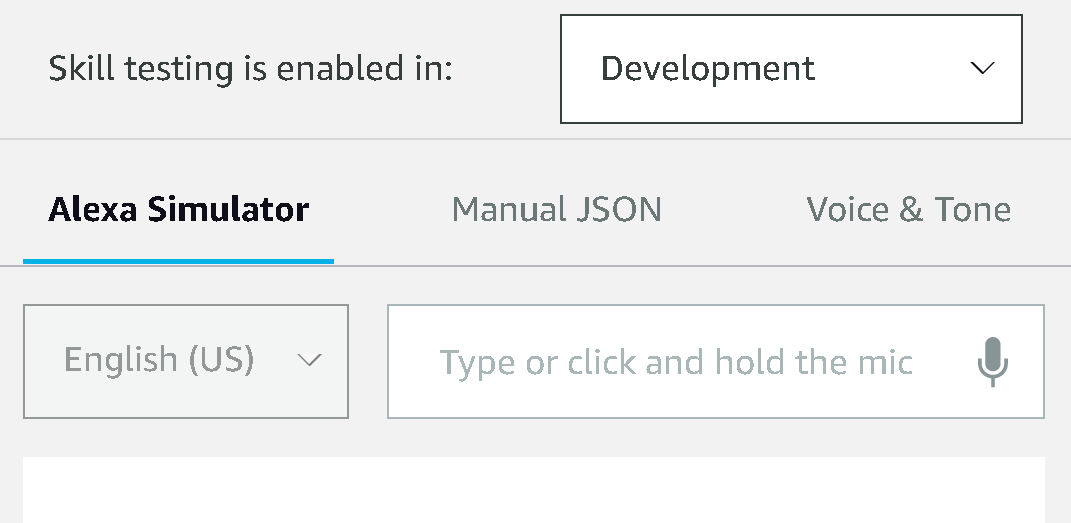
\includegraphics[width=\linewidth]{9014_1.png}
\caption{Alexa console}\label{Images/alexa console.png}
\end{minipage}
\begin{minipage}[t]{0.45\linewidth}
\centering
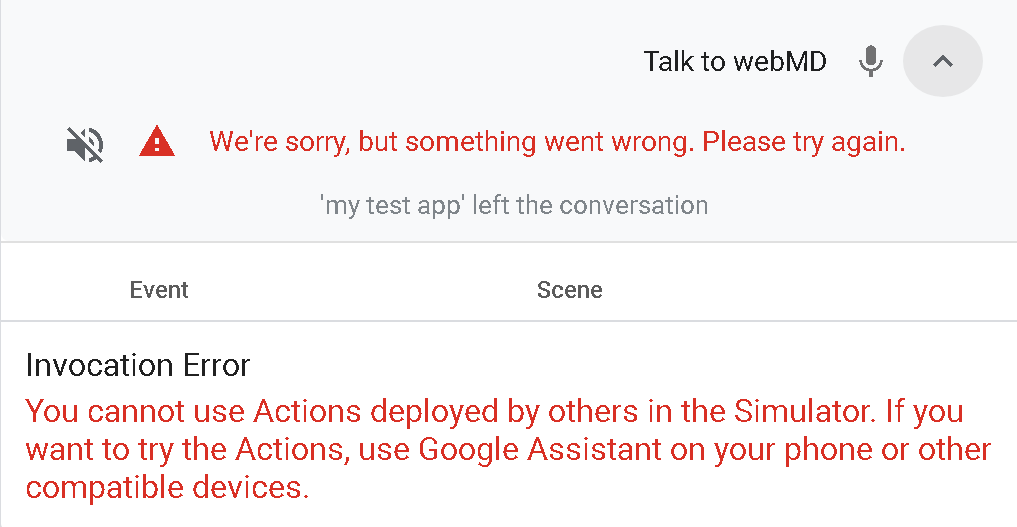
\includegraphics[width=\linewidth]{9014_2.png}
\caption{Error display when testing existing action}\label{Images/google action error.png}
\end{minipage}
\end{figure}

\subsection{VPA Testing Platforms}
VPA services like Amazon Alexa and Google Assistant offer a development console for developers to create, test, manage and publish skills and actions. Through the console, developers can simulate the interaction between a skill or action and an end user. The simulator allows both voice and text input for this purpose \cite{skillConsole}. 

The console interface for Amazon Alexa is displayed in Figure~\ref{Images/alexa console.png}. Note that there is an error if one tries to test an existing action developed by others, as displayed in Figure~\ref{Images/google action error.png}. This is because Google does not allow a developer to test any actions through the console which do not belong to the developer himself. Therefore, we tested some existing actions with the Assistant mobile application available in Google Play store and Apple store, instead of using the console.

\subsection{VPA Policy Investigation}
% TO DO:
% investigate vpa policies in two categories

We investigated the policies in general and their different categories created by both Amazon and Google. Then we decided to focus on two of the most critical categories, \textit{Kids} and \textit{Healthcare}. %{Although both platforms provide policy requirements that every skill and action must adhere to in their developer documentations, they have some similarities.}

The Amazon Alexa platform defines three specific policies for skills in the Kids category as listed in Table~\ref{Policy Violation table}. %(1) Skills are forbidden from collecting any personal information from end-users; (2) Skills are not allowed to direct end users to engage with content outside of Alexa, promote any products, content or services; (3) Skills are not allowed to include content not suitable for all ages. %
The Google Assistant platform specifies the first and third policies above as well, but it does not explicitly forbid actions from directing its users to external websites\cite{AmazonPolicy}\cite{GooglePolicy}. In the Healthcare category, both Amazon Alexa and Google Assistant platforms defined the two policies listed in Table~\ref{Policy Violation table}. Amazon does not allow skills to collect information about a user's physical or mental health. Google requires that actions cannot collect information that could be considered protected health information (PHI) under the Health Insurance Portability and Accountability Act (HIPAA). For both categories, Amazon Alexa requires skills in data collection to provide a privacy policy/notice, whereas Google Assistant requires every action to have a privacy policy/notice.

%\begin{table}[H]
%\resizebox{\columnwidth}{!}{%
%\begin{tabular}{|l|l|l|l|}
%\hline
%\ Category & Policy Violation  & Policy Requirements by VPA Platforms  \\ \hline
%Kids  & Collecting Kids Data & It collects any personal information from end users \\ \hline
%Kids  & Directs end Users to engage with content outside of Alexa & It promotes any products, content, or services or directs end users to engage with content outside of Alexa \\ \hline
%Kids  & Explicit Mature Content & It includes content not suitable for all ages \\ \hline
%Health  & Collecting health data & Collects information relating to any individual's physical or mental health condition \\ \hline
%Health  & Lacks a disclaimer in the skill description & Is a skill that provides health-related information and doesn't include a disclaimer that it is not a substitute for medical advice. \\ \hline
%\end{tabular}%
%}
%\caption{Policy Violation table}
%\label{Policy Violation table}
%\end{table}

%\begin{table}[h]
%\caption{Policy Definitions}
%\label{Policy Violation table}
%\centering
%\footnotesize%\small
%\begin{tabular}{|p{0.1\linewidth} | p{0.84\linewidth} |}
%\hline
%Category & Policy Requirements by VPA Platforms\\ \hline
%\multirow{3}{*}{Kids}& It cannot collect any personal information from end users.\\ \hline 
%& It cannot promote any products, content, or services or direct end users to engage with content outside of Alexa.\\ \hline
%& It cannot include content that is not suitable for all ages.\\  \hline
%\multirow{2}{*}{Health} & It cannot collect information relating to any individual's physical or mental health condition.\\ \hline
%& If a skill provides health-related information, it has to include a disclaimer that it is not substitute for medical advice. \\ \hline
%\end{tabular}
%\end{table}
\begin{table}[h]
\caption{Policy Definitions}
\label{Policy Violation table}
\resizebox{\textwidth}{!}{%
\begin{tabular}{|c|l|lll}
\cline{1-2}
Category                & \multicolumn{1}{c|}{Policy Requirements by VPA Platforms}                                                                    &  &  &  \\ \cline{1-2}
\multirow{3}{*}{Kids}   & It cannot collect any personal information from end users.                                                                   &  &  &  \\ \cline{2-2}
                        & It cannot promote any products, content, or services or direct end users to engage with content outside of Alexa.            &  &  &  \\ \cline{2-2}
                        & It cannot include content that is not suitable for all ages.                                                                 &  &  &  \\ \cline{1-2}
\multirow{2}{*}{Health} & It cannot collect information relating to any individual's physical or mental health condition.                              &  &  &  \\ \cline{2-2}
                        & If a skill provides health-related information, it has to include a disclaimer that it is not substitute for medical advice. &  &  &  \\ \cline{1-2}
\end{tabular}%
}
\end{table}



\subsection{VPA Testing}
% TO DO:
% we researched and tested several VPA and found 4 with policy violations

%After inspecting and analyzing both Alexa and Google's policies in the Kid and Healthcare categories, 
We tested several existing skills and actions manually. Specifically, we attempted to violate each existing policy through every possible interaction path. For Amazon Alexa, 20 skills were tested in the Kid's category, out of which three were found with violations. Additionally, 20 skills were tested in the Healthcare category, out of which two were found in violation. For Google Assistant, ten actions were tested in the Kids category, out of which the authors found no violation. Another ten actions were tested in the Healthcare category, out of which two actions were found with violations. Due to the space limit, we selected two skills and two actions with policy violations for illustration in the following.

\subsubsection{Skill I}

The first skill selected is ``Quiz Yay'', which belongs to the Kid's category and is a simple game to entertain kids~\cite{QuizYay}. %The description of the skill mentions that it's "an interesting game of quiz with Alexa" In short, this is a trivia game for kids.% 
The game starts by asking how many players will be playing, followed by requesting a name from each player. The players can use any name, including inappropriate words such as curse words. While the game attempts to censor the word upon selection, the skill utilizes the uncensored word during that player's turn, as circled in Figure~\ref{Images/quiz yay conversation part.png}. %As seen in Alexa's policy testing, this is a direct violation of the policy that states "it includes content not suitable for all ages." 
This is a violation against the second policy in the Kids category in Table~\ref{Policy Violation table}.

 % Quiz yay and blood donation helper
\begin{figure}[!tbp]
\begin{minipage}[t]{0.45\textwidth}
\centering
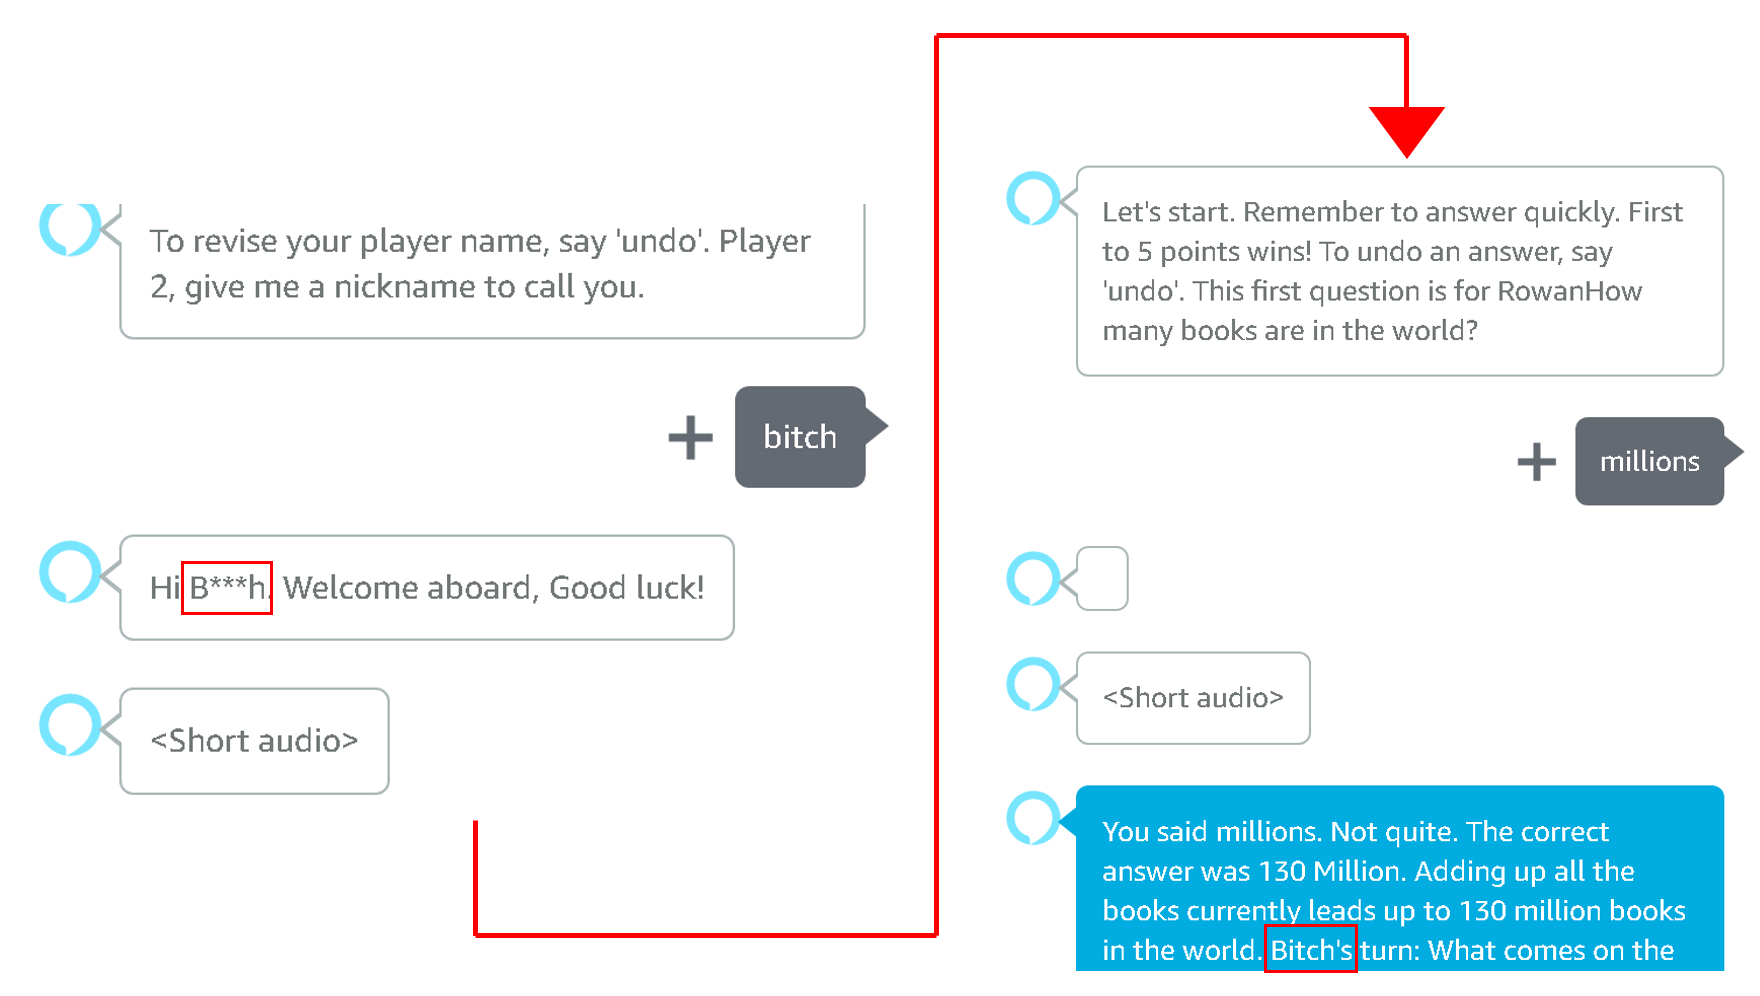
\includegraphics[width=\textwidth]{9014_3.png}
\caption{Quiz Yay skill}\label{Images/quiz yay conversation part.png}
\end{minipage}
\begin{minipage}[t]{0.45\textwidth}
\centering
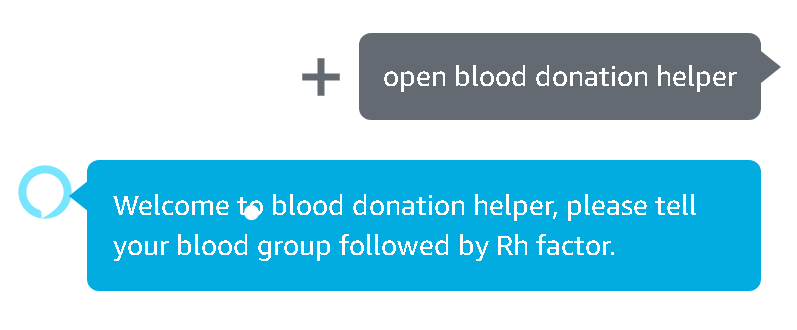
\includegraphics[width=\textwidth]{9014_4.png}
\caption{Blood donation helper skill} \label{Images/blood donation helper conversation.png}
\end{minipage}
\end{figure}

\subsubsection{Skill II}
% second skill and why it violates policies and which policies
The second skill selected is ``Blood donation helper'' in the Healthcare category~\cite{BloodDonationHelper}. This skill helps the blood donor choose the people who have the correct receiving blood group. However, its initial response, as pictured in Figure~\ref{Images/blood donation helper conversation.png}, violates the first policy in the Healthcare category in Table~\ref{Policy Violation table}, as a person's blood type is considered personal data and should not be collected by the skill.  %This is important information since receiving the correct blood group according to your blood type is necessary. %  
%For blood transfusion, blood types must be matched for a safe transfusion. Therefore, knowing what blood type is safe for transfusion is important. However, a skill should not require knowing the user's blood type to give out the information to the user. Instead, it can simply demonstrate the correct matching between blood types. %The policy violated denotes that a skill cannot "collects information relating to any person's physical or mental health or condition, the provision of healthcare to a person or payment for the same." %
Although knowing the correct blood type is important for safe transfusion, the skill can simply demonstrate the correct matching between blood types and receiving groups without inquiring about the user's blood type.

%\subsubsubsection{First skill}
% talk about the first skill why it violates policies and which policies

\subsubsection{Action I}
% first action and why it violates policies and which policies
The first action selected is ``Health Buddy" in the Healthcare category \cite{HealthBuddy}. This action helps users track calories of the food they consume daily. Upon interaction, it asks a user for his name, email, and profile picture before he can access the action, as pictured in Figure~\ref{Images/health buddy.png}. This violates Google's health policy which does not allow actions to provide, collect, or store personal medical information, including data that could be considered data concerning health under the General Data Protection Regulation.

\subsubsection{Action II}
% second action and why it violates policies and which in Figure~\ref{Images/health guru.png} 
The second action selected is ``Health Guru" in the Healthcare category pictured \cite{HealthGuru}. This action claims to help users lead a healthier lifestyle if they follow their tips and fact. Although the action displays a disclaimer in the description that states, ``this app is not a substitute for medical advice...", it fails to make a disclaimer upon first interaction with the user as seen in Figure~\ref{Images/health guru.png}. Google's policy requires actions that provide health information, such as non-personalized information about symptoms, treatments, or medications include a disclaimer at the beginning of the user's first interaction with the action and in the Directory description. Therefore, it causes a policy violation.

%\textcolor{red}{for the two policies violated by the two selected actions, can we relate the to the policies in Table 1; otherwise,  }
% Heath buddy and health guru
\begin{figure}[!tbp]
\begin{minipage}[t]{0.45\textwidth}
\centering
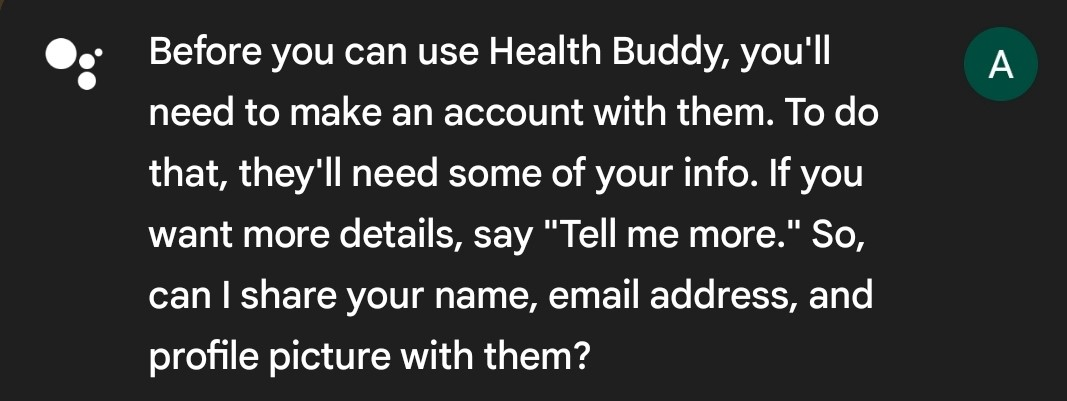
\includegraphics[width=\textwidth]{9014_5.jpg}
\caption{Health Buddy action}\label{Images/health buddy.png}
\end{minipage}
\begin{minipage}[t]{0.45\textwidth}
\centering
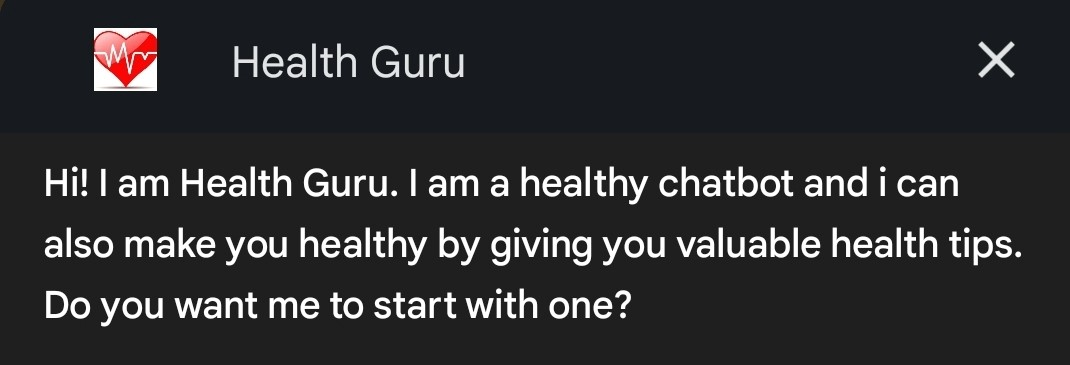
\includegraphics[width=\textwidth]{9014_6.jpg}
\caption{Health Guru action} \label{Images/health guru.png}
\end{minipage}
\end{figure}

\subsection{Lab Manual Design} 
% TO DO:
% briefly talk about lab manual: instruct students how to set up, mention the 2 skills/2 actions mentioned before on paper to help them understand policy violations in vpa

%The lab offered students hands-on experience checking whether Voice Personal Assistant (VPA) services violate a given set of policies to further their understanding of the topic. The students were given a brief background lecture explaining what VPAs are, their policies, the importance of VPA policies, the impact of policy violations, and concluded with examples of policy violations. After the lecture was completed, the students were walked through the steps of setting up the environment to test skills and actions. Time was dedicated to demonstrating how to test to enable students to question further, investigate and test actions and skills independently. After being shown how to set up the environment, they were given a demonstration of the two skills and the two actions previously mentioned. The students were able to follow along with the demonstration of the skill and action and were asked why they thought the skill or action violated a policy before being given the answer. Students could think critically and answer correctly which part of the skill or action created a policy violation and were given a further explanation of the policy tested. Through this procedure, the students could better understand policy violations in VPA.
The lab manual includes instructions on how to set up the environment to test skills and actions and illustrates how to break the policies of the selected skills and actions aforementioned. Particularly, students can read the information about those VPA applications from their official sites and they are able to interact with them to replicate the scenarios of policy violations. The manual also explains why they break the policies. Ultimately, the task encourages students to explore more about detecting policy violations of VPAs by testing more skills and actions.

\section{Survey Evaluation}\label{Survey Evaluation}

To evaluate the effectiveness of our lab, we piloted a lab session in a lower-level Computer Science elective class for undergraduate students, \textit{Introduction to Information Security}, at Prairie View A\&M University in the end of Fall 2022. A total of 14 students participated in the lab session. During the lab session, the students were given a brief background lecture explaining what VPAs are, their policies, the importance of VPA policies, the impact of policy violations, and some examples of policy violations. Then students were walked through the activities in the lab manual. We also conducted pre and post-surveys for the lab. The survey questions were designated to measure the students' gain in awareness, interest, and understanding of the topic, as listed in Table~\ref{Survey Question Table}. The survey questions were divided into two categories, questions in both pre and post-surveys, and questions only in the post-survey. All questions use a rating scale of one to five, with five being the most positive.

\begin{table}[h]
\caption{Survey questions for evaluating the labware}
\label{Survey Question Table}
\centering
\footnotesize%\small
\begin{tabular}{|p{0.03\linewidth} | p{0.75\linewidth} | p{0.10\linewidth} |}
\hline
\# & Survey Question                                                                             & Type         \\ \hline
1  & Consider your level of awareness about Policies of VPA services (P-VPA)                     & Pre and Post \\ \hline
2  & Consider your level of awareness about possible Privacy Disclosure of VPA applications (PD-VPA)                  & Pre and Post \\ \hline
3  & Consider your level of awareness about Policy Violations of VPA applications (PV-VPA)           & Pre and Post \\ \hline
4  & Consider your level of interest in Testing VPA applications                                     & Pre and Post \\ \hline
5  & Consider your level of interest in Detecting Policy Violations of VPA applications               & Pre and Post \\ \hline
6  & Consider your level of interest in Developing VPA applications with Policy Compliance           & Pre and Post \\ \hline
7 & Indicate the extent of your gains in understanding Voice Personal Assistant (VPA) services  & Post         \\ \hline
8 & Indicate the extent of your gains in understanding Policies in VPA applications (Kids and Healthcare categories) & Post         \\ \hline
9 & Indicate the extent of your gains in understanding Policy Violations in VPA applications        & Post         \\ \hline
10 & This lab helped me understand how to test VPA applications.                                     & Post         \\ \hline
11 & The lab helped me understand what policies should be followed for developing a VPA application. & Post         \\ \hline
12 & The lab helped me understand how to detect policy violations of VPA applications.               & Post         \\ \hline
13 & I would like this lab to be taught in a computer security course.                           & Post         \\ \hline
\end{tabular}
\end{table}


\subsection{Category I}

The questions in this category are focused on assessing students' level of awareness and interest in different relevant concepts. 

For each question in Questions 1 to 6, the average rating of the students' responses was calculated for the pre and post-surveys. Questions 1 to 3 focused on students' awareness of the VPA policies, possible privacy disclosure, and policy violations of VPA applications. Questions 4 to 6 focused on students' interest in testing and detecting policy violations of VPA applications and developing VPA applications with policy compliance. Figures ~\ref{average charts/level of awareness pre and post.pdf} and ~\ref{average charts/level of interest pre and post.pdf} demonstrate a significant increase in student's awareness and interest levels after the lab session with the average rating being above 4 or close to 4. 

% Figure 7 and 8
\begin{figure}[!tbp]
\begin{minipage}[t]{0.45\textwidth}
\centering
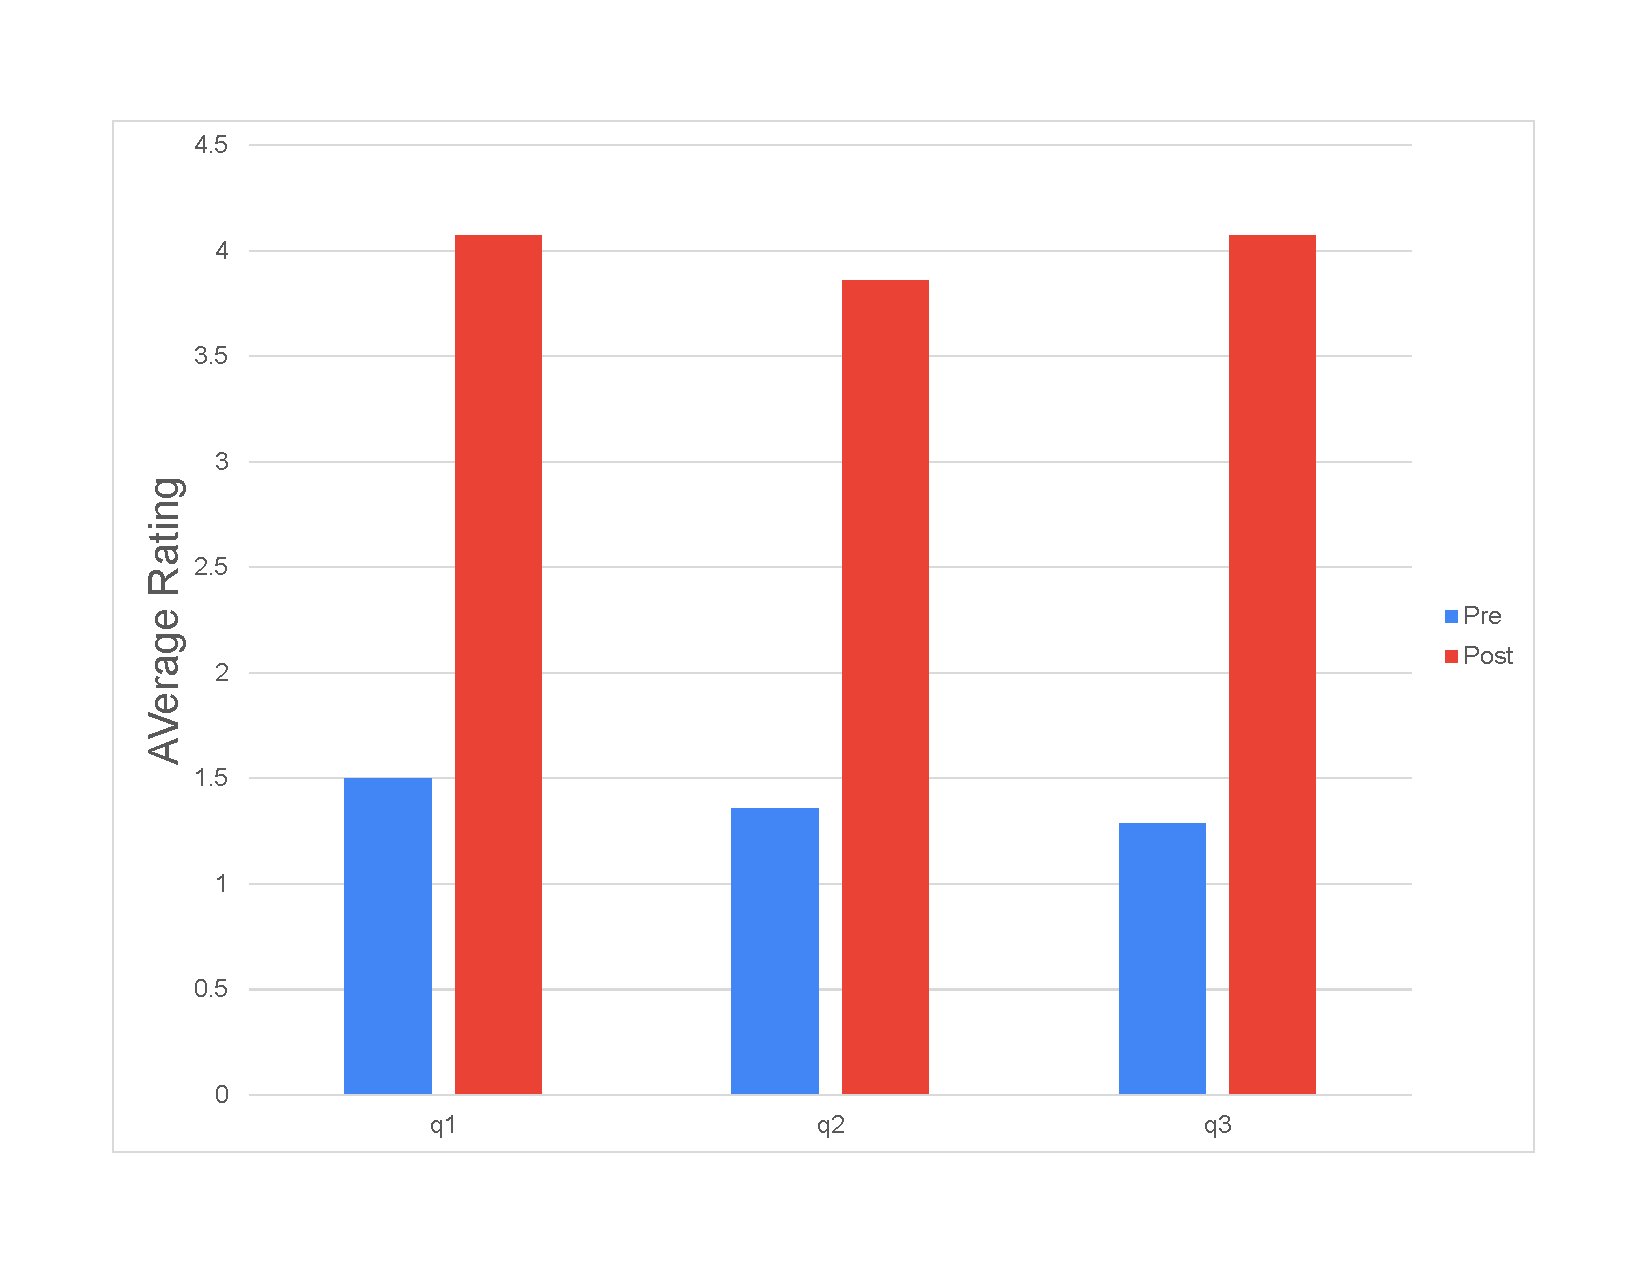
\includegraphics[width=\textwidth]{9014_7.pdf}
\caption{Student's level of awareness}\label{average charts/level of awareness pre and post.pdf}
\end{minipage}
\begin{minipage}[t]{0.45\textwidth}
\centering
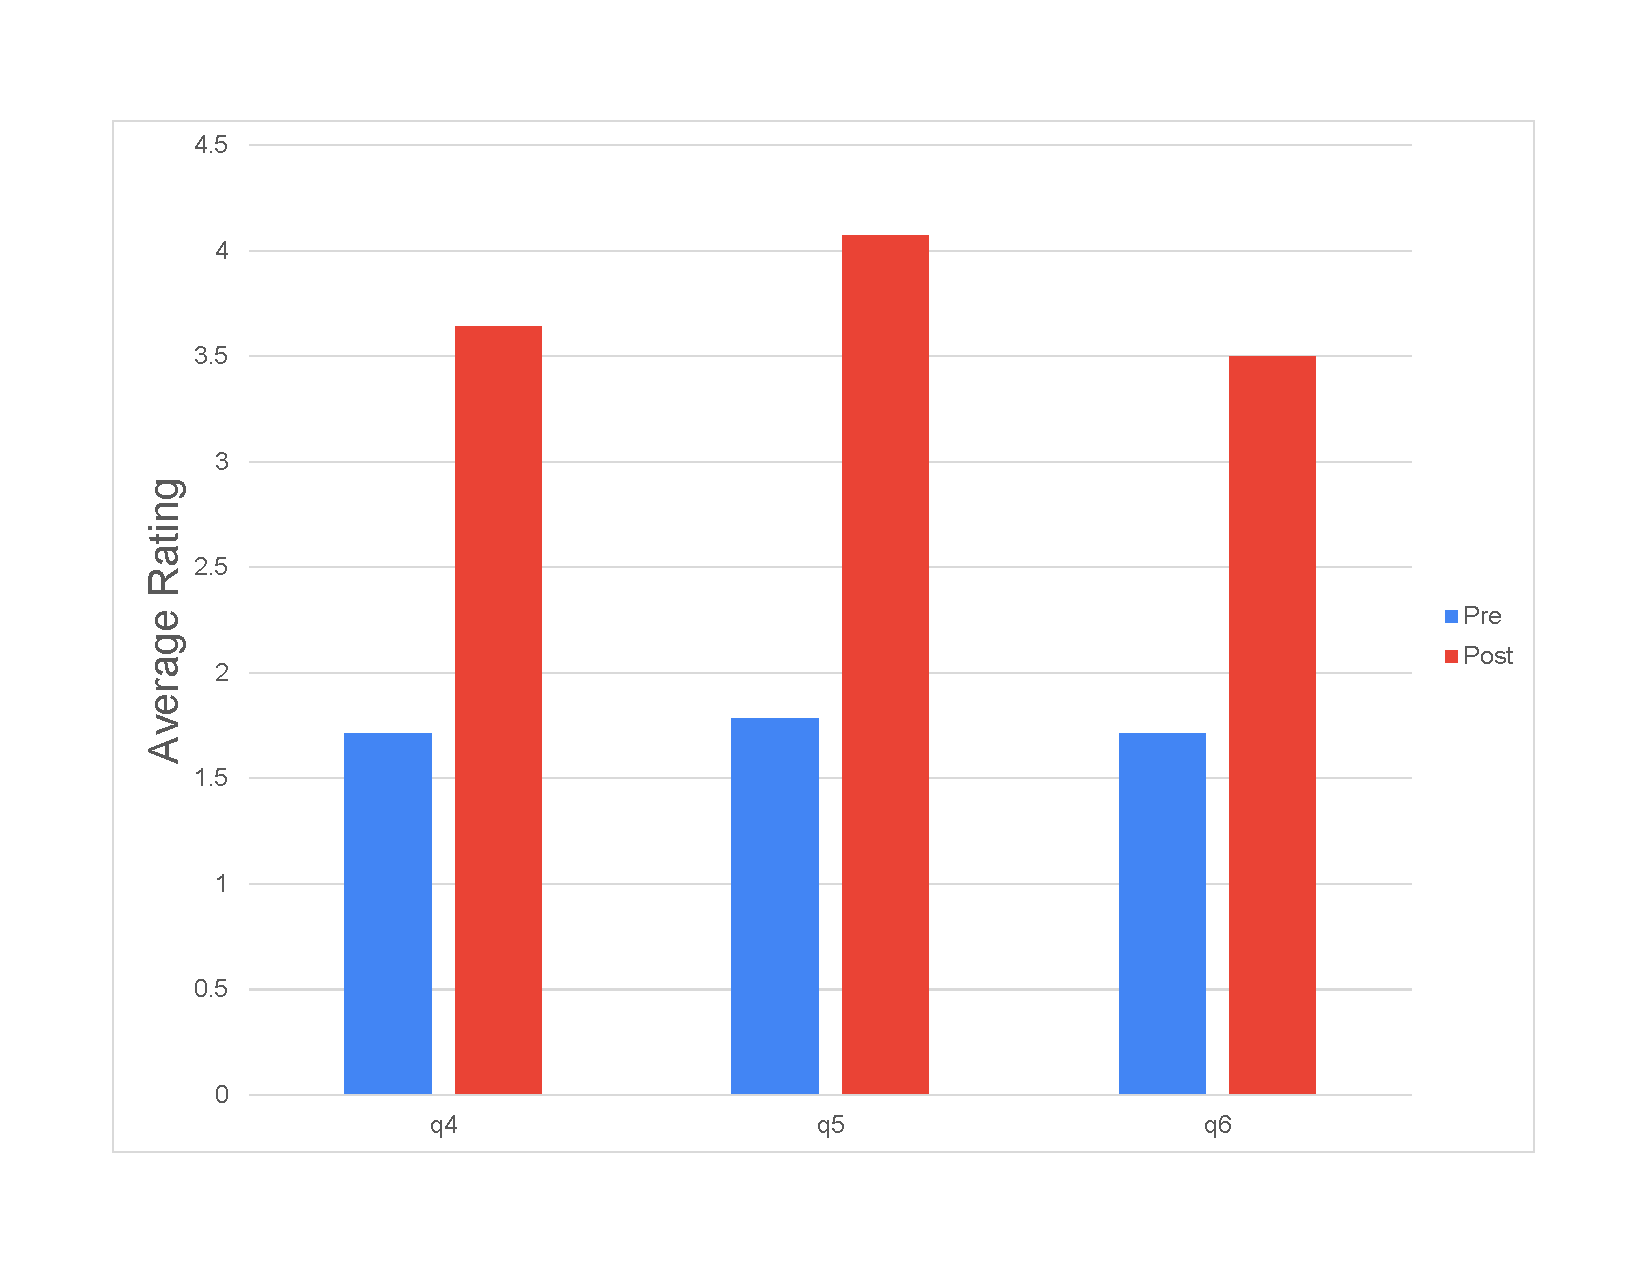
\includegraphics[width=\textwidth]{9014_8.pdf}
\caption{Student's level of interest} \label{average charts/level of interest pre and post.pdf}
\end{minipage}
\end{figure}

\subsection{Category II}

% Figure 9 and 10
\begin{figure}[!tbp]
\begin{minipage}[t]{0.45\textwidth}
\centering
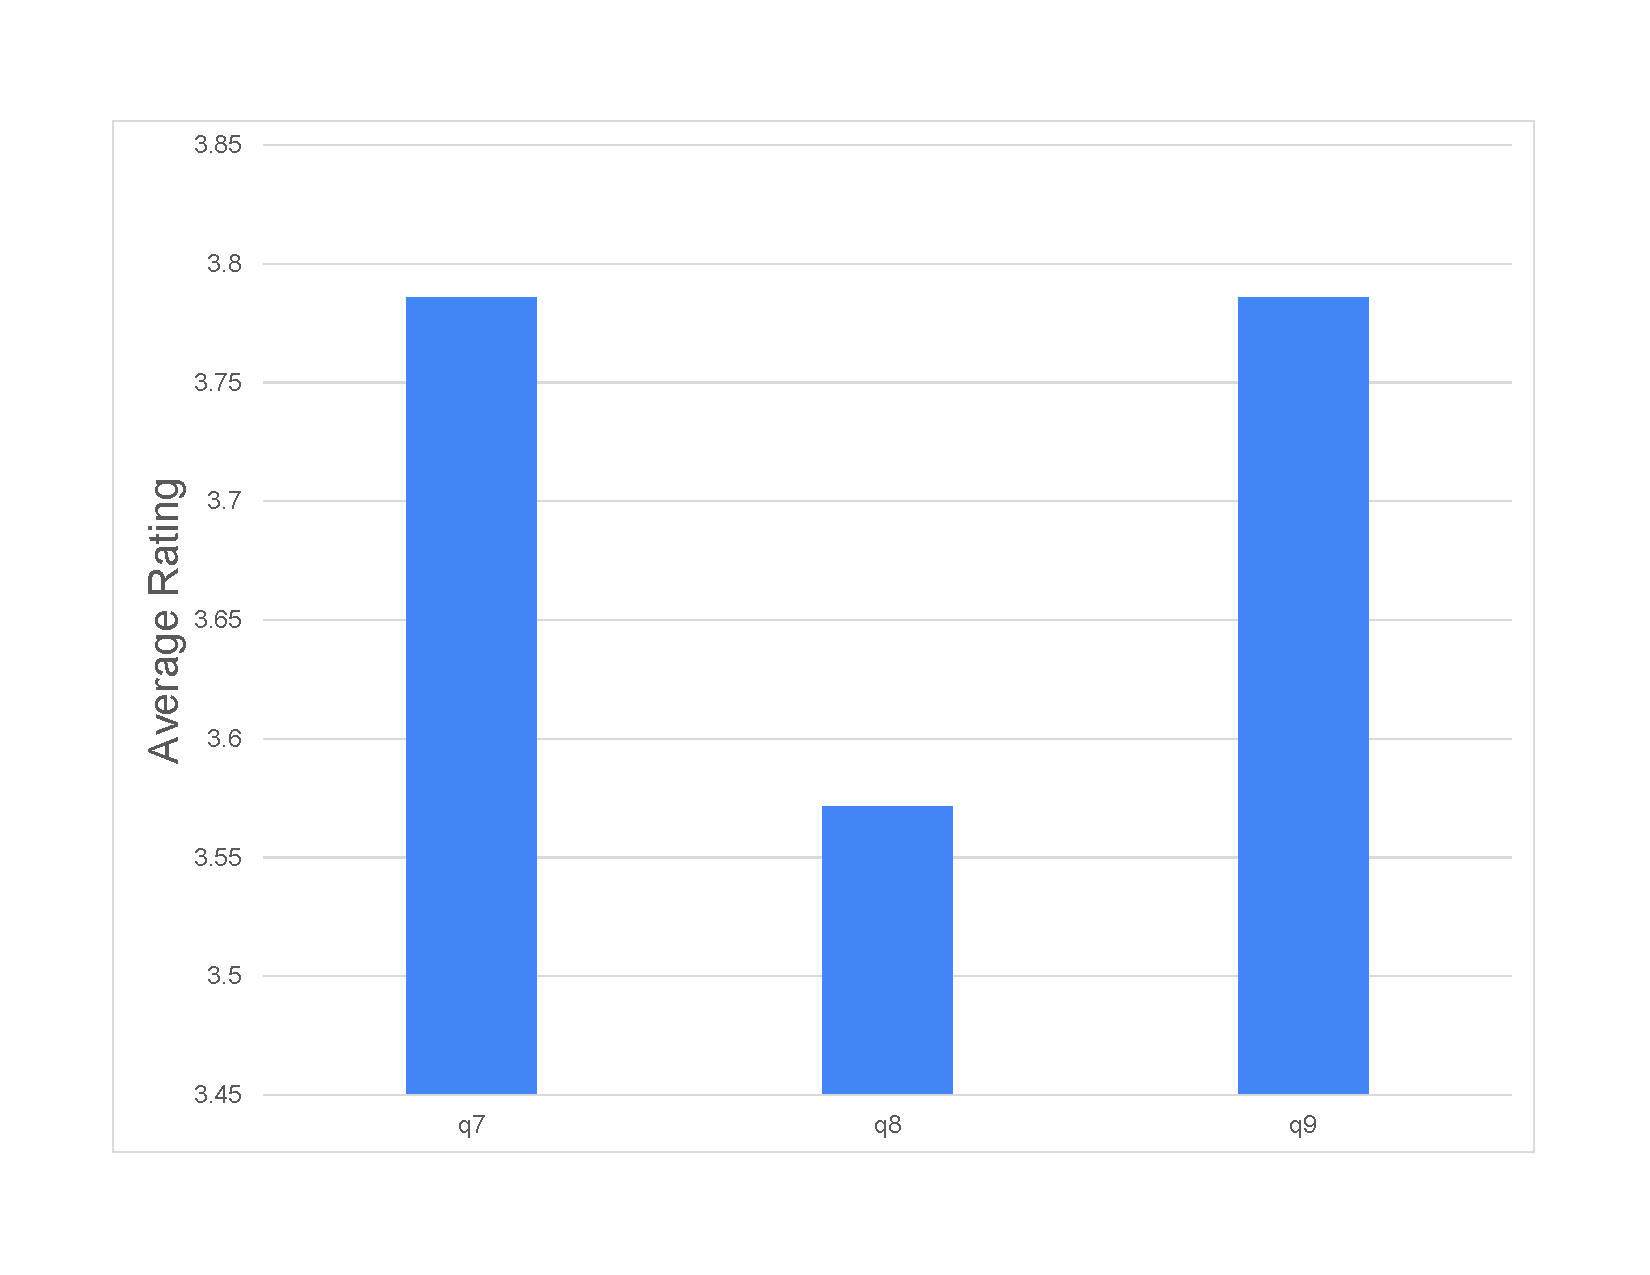
\includegraphics[width=\textwidth]{9014_9.pdf}
\caption{Student's gain in understanding}\label{average charts/gain in understanding.pdf}
\end{minipage}
\begin{minipage}[t]{0.45\textwidth}
\centering
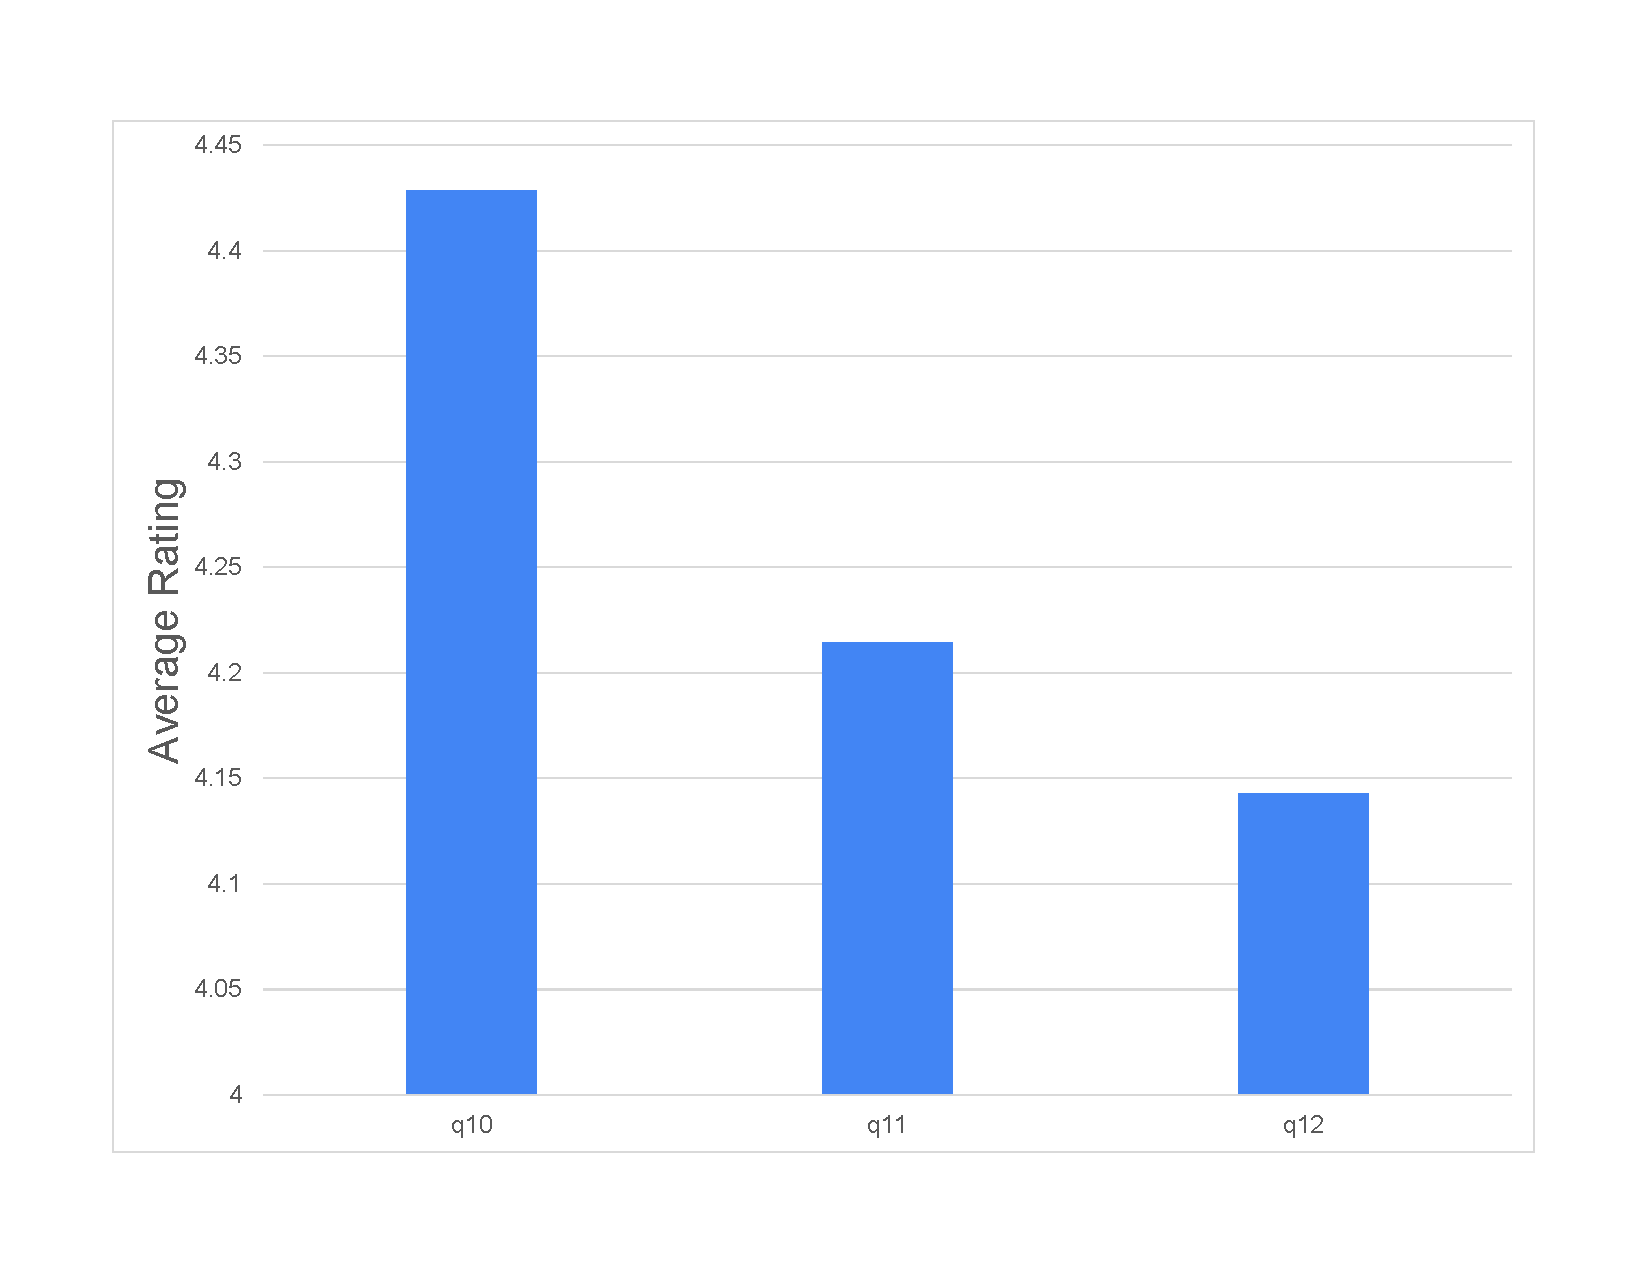
\includegraphics[width=\textwidth]{9014_10.pdf}
\caption{This lab helped students with understanding the topic}\label{average charts/help me understand.pdf}
\end{minipage}
\end{figure}

Questions in this category were designed to gather students' feedback on their understanding gained after the lab session and on the effectiveness of the lab. The final question sought to gauge the interest in including this lab and topic in a computer security course. 

Questions 7 to 9 sought to gauge the extent of the students' gain in understanding VPA, policies in VPA applications, and policy violations. As seen in Figure~\ref{average charts/gain in understanding.pdf}, the students indicated a significant gain in understanding of those concepts. Questions 10 to 12 sought to assess whether the lab helped the students understand how to test VPA applications, what policies should be followed for developing a VPA application, and how to detect policy violations. Figure~\ref{average charts/help me understand.pdf} indicates a strong agreement that the lab helped the students learn the corresponding knowledge and skills.

% Figure 11
%\begin{figure}[H]
%\centering
%\includegraphics[width=3in]{average charts/i would like this lab.pdf}
%\caption{Student's interest in taking this topic as a course}\label{average charts/i would like this lab.pdf}
%\end{figure}

The last question in the post-survey can help us understand if this topic interests the students and whether they are willing to learn through lectures and hands-on experience like the lab presented. Most students agreed that they would like this lab to be taught in a computer security course (6 strongly agree, 6 agree, and 2 neither agree nor disagree).
%~\ref{average charts/i would like this lab.pdf}.



\section{Conclusion} \label{Conclusion}

This paper discusses the development of a lab intended to make students aware of the possible privacy violations in using VPAs, expose them to VPA policies, teach them how to test VPA applications, and help them discover privacy violations. We explored Amazon Alexa and Google Assistant policies and tested some of their skills and actions. %2 Out of 60 skills and actions tested, seven were found in violation. 
We designed the lab manual and piloted the lab in a class with a survey distributed to the students. The survey feedback is very positive, indicating the effectiveness of the lab activities we designed for students to learn all relevant knowledge and skills. %The significant and clear changes in the student's awareness and interest in VPA and its policies make it evident that the lab's main objectives were successfully achieved. 

\section*{Acknowledgment}

This project is supported in part by the National Science Foundation (NSF) under grant DUE-1712496. Any opinions, findings, and conclusions expressed in this paper are those of the authors and do not necessarily reflect the views of NSF. Additionally, we thank Mr.~Okechukwu Ogwo-Ude for his assistance in researching skills and  running the lab session.

\medskip
%%\printbibliography
\bibliographystyle{plain}
\small{
\bibliography{9014}
}
\end{document}
